\documentclass[11pt,a4paper]{article}
\usepackage[utf8]{inputenc}
\usepackage[T1]{fontenc}
\usepackage[brazil]{babel}
\usepackage{lmodern}
\usepackage{amsmath,amssymb,bm}
\usepackage{graphicx,booktabs,float,geometry,url,array,xcolor,caption}
\usepackage[hidelinks]{hyperref}
\geometry{margin=2.2cm}
\captionsetup{font=small}
\emergencystretch=2em
\providecommand{\versao}{sem versão}
% gerado por gera_dados.py; nao edite
\newcommand{\nCasos}{6}
\newcommand{\nTot}{15440}
\newcommand{\nFORMtot}{56}
\newcommand{\nLStot}{3964}
\newcommand{\nMCtot}{11300}
\newcommand{\nTreze}{120}
\newcommand{\nFormConv}{1}
\newcommand{\anPorLinha}{2{,}89}
\newcommand{\fsDetZero}{1{,}524}
\newcommand{\fsDetVinte}{0{,}907}
\newcommand{\fsDetSetenta}{1{,}184}
\newcommand{\huZero}{1{,}583}
\newcommand{\huVinte}{0{,}929}
\newcommand{\huSetenta}{1{,}248}
\newcommand{\huSdZero}{0{,}165}
\newcommand{\huSdVinte}{0{,}091}
\newcommand{\huSdSetenta}{0{,}130}
\newcommand{\difZero}{$-$3{,}7}
\newcommand{\difVinte}{$-$2{,}3}
\newcommand{\difSetenta}{$-$5{,}1}
\newcommand{\ksBaixoVinte}{1{,}104}
\newcommand{\triDoisVinte}{0{,}915}
\newcommand{\triTresVinte}{0{,}908}
\newcommand{\triQuatroVinte}{0{,}907}
\newcommand{\triTresIXII}{1{,}296}
\newcommand{\triQuatroIXII}{1{,}281}
\newcommand{\vertical}{0{,}983}
\newcommand{\inclinadaTri}{0{,}908}
\newcommand{\fsNoventaDois}{0{,}855}
\newcommand{\fsNoventaTres}{0{,}793}
\newcommand{\sdZero}{0{,}062}
\newcommand{\muZero}{1{,}507}
\newcommand{\razaoSdZero}{0{,}38}
\newcommand{\sdVinteMC}{0{,}036}
\newcommand{\razaoSdVinte}{0{,}40}
\newcommand{\cvHuZero}{10{,}4}
\newcommand{\cvNossoZero}{4{,}1}
\newcommand{\cvHomZero}{8{,}0}
\newcommand{\cvHomVinte}{6{,}5}
\newcommand{\cvHuVinte}{9{,}8}
\newcommand{\wcZero}{0{,}20}
\newcommand{\wcVinte}{0{,}41}
\newcommand{\pfHomVinte}{94{,}1}
\newcommand{\homFora}{0{,}00}
\newcommand{\huNormalCinquenta}{78{,}5}
\newcommand{\huNormalTrinta}{18{,}2}
\newcommand{\nossoNormalTrinta}{7{,}06}
\newcommand{\pfLSTrinta}{7{,}12}
\newcommand{\cvLSTrinta}{4{,}7}
\newcommand{\pfMCTrinta}{6{,}75}
\newcommand{\nfMCTrinta}{135}
\newcommand{\nMCTrinta}{2000}
\newcommand{\linhasTrinta}{109}
\newcommand{\anLSTrinta}{272}
\newcommand{\zTrinta}{+0{,}6}
\newcommand{\pfLSTrintaSeis}{0{,}268}
\newcommand{\cvLSTrintaSeis}{4{,}9}
\newcommand{\pfMCTrintaSeis}{0{,}325}
\newcommand{\nfMCTrintaSeis}{13}
\newcommand{\nMCTrintaSeis}{4000}
\newcommand{\linhasTrintaSeis}{491}
\newcommand{\anLSTrintaSeis}{1365}
\newcommand{\zTrintaSeis}{-0{,}6}
\newcommand{\nMCEquivTrintaSeis}{158.000}
\newcommand{\razaoTrintaSeis}{115}
\newcommand{\nMCEquivTrinta}{5.900}
\newcommand{\razaoTrinta}{21}
\newcommand{\pfLSQuarenta}{0{,}072}
\newcommand{\cvLSQuarenta}{11{,}8}
\newcommand{\pfMCQuarenta}{0{,}125}
\newcommand{\nfMCQuarenta}{5}
\newcommand{\pfFORMQuarenta}{0{,}012}
\newcommand{\pfLSCinquenta}{99{,}77}
\newcommand{\pfMCCinquenta}{99{,}67}
\newcommand{\zMax}{0{,}9}
\newcommand{\nZ}{4}
\newcommand{\mcTrezeOk}{6}
\newcommand{\mcTrezeN}{20}
\newcommand{\mcTrezeDif}{0{,}0000}
\newcommand{\cvNossoMin}{3{,}8}
\newcommand{\cvNossoMax}{4{,}2}
\newcommand{\linhaTeto}{12}

\title{Caso A da chuva: Hu et al.\ (2024)\\ FORM modal, line sampling e Monte Carlo contra o artigo}
\author{Diogo Cecílio}
\date{23/11/2026 --- versão \versao}
\begin{document}
\maketitle
\begin{abstract}
O caso A é o talude de 10~m sob chuva de Hu et al.~\cite{hu2024}. Ele rodou no fermi em \nCasos{} cenários de chuva
(campanha \texttt{hu2024}, $k_s = 2 \times 10^{-5}$~m/s). Cada cenário tem o FORM modal, o line sampling (LS) e o Monte
Carlo direto, num total de \nTot{} análises do MEF. Com as médias, o nosso FS determinístico fica de 2 a 5\,\% abaixo
da média de Hu ($\fsDetZero$, $\fsDetVinte$ e $\fsDetSetenta$ em 0, 24 e 72~h a 50~mm/h por 24~h). O LS concorda com o
MC direto nos \nZ{} cenários em que o MC tem falhas ($|z| \le \zMax$). A 30~mm/h por 24~h, por exemplo, o LS dá
$\pfLSTrinta\,\%$ e o MC dá $\pfMCTrinta\,\%$. As $P_f$ de Hu, porém, não se reproduzem: o desvio do nosso FS é
$\approx \razaoSdZero$ do dele ($\sdZero$ contra $\huSdZero$ em 0~h). O $CoV$ dele (\cvHuZero\,\%) passa até do limite
homogêneo (\cvHomZero\,\%), o de $c'$ e $\varphi'$ como variáveis aleatórias, sem campo. Numa aproximação normal, a
média e o desvio de Hu reproduzem a $P_f$ dele, e os nossos reproduzem a nossa. Logo, a diferença está no espalhamento
do FS e não no método de confiabilidade. Em todos os cenários, o menor FS da história cai no fim da chuva. O caso A
serve, então, como verificação determinística e como teste do LS contra o nosso próprio MC, mas não como referência de
$P_f$.
\end{abstract}
\tableofcontents

\section{O que foi rodado}\label{sec:rodado}
\begin{itemize}
  \item \textbf{O problema~\cite{hu2024}:} talude de 10~m a $45^\circ$ num domínio de $70 \times 20$~m, com os seis
    pontos $(0;0)$, $(70;0)$, $(70;10)$, $(40;10)$, $(30;20)$ e $(0;20)$. O nível d'água é horizontal na cota 5~m. A
    sucção inicial é hidrostática a partir do nível, com teto de 50~kPa. A lateral esquerda e a base são impermeáveis,
    e a direita tem carga de 5~m. As leis hidráulicas são de van Genuchten--Mualem ($\theta_s = 0{,}399$,
    $\theta_r = 0{,}024$, $\alpha = 0{,}0357$~kPa$^{-1}$, $n = 1{,}71$, lidos da Fig.~4), com $k_s = 2 \times
    10^{-5}$~m/s, o valor do texto. A resistência é a de Vanapalli, com $\chi = S_e$, e $\gamma = 17{,}8$~kN/m$^3$.
  \item \textbf{Os campos:} $c'$ (média 8~kPa, $CoV = 0{,}15$) e $\varphi'$ (média $24^\circ$, $CoV = 0{,}10$) são
    log-normais. O núcleo é $\exp(-|\Delta x|/20 - |\Delta y|/2)$, e a correlação entre as normais é
    $\rho(c', \varphi') = -0{,}5$. Os campos vêm da base de Nyström no domínio do talude~\cite{formulacao}: grade de
    $0{,}3 \times 0{,}1$~m (34\,950 nós) e $M = 150$ termos por campo, que retêm 0,869 da variância (0,831 com 100
    termos e 0,892 com 200). O $k_s$ é determinístico, então um transiente por cenário serve a todas as realizações.
  \item \textbf{As malhas:} o transiente roda na \texttt{TriGMesh} de nível 4 (tri4, 27\,700 equações, $dt = 0{,}1$~h
    até 72~h, $\approx 18$~min por cenário). O FS vem do SRM na \texttt{TriGMesh(1)}, com 4 níveis adaptativos em $h$,
    no fim da chuva $D$ e em $D + 6$~h. A falha é o menor FS abaixo de 1 (primeira passagem).
  \item \textbf{Os métodos:}
    \begin{itemize}
      \item \emph{FORM modal:} HLRF~\cite{hasofer1974,rackwitz1978} com o gradiente modal do SRM~\cite{formulacao},
        até 10 iterações de uma análise cada. Convergiu em \nFormConv{} dos \nCasos{} cenários; nos outros, parou nas
        10 iterações (Seção~\ref{sec:prob}).
      \item \emph{Line sampling~\cite{koutsourelakis2004}:} na direção do FORM, com semente 7. Para no primeiro
        $N \ge 30$ com $CoV(P_f) \le 5\,\%$, até 600 linhas, ou até 60 linhas quando $\beta > 5$. Cada linha custa
        \anPorLinha{} análises em média.
      \item \emph{Monte Carlo direto:} de 300 a 4000 realizações por cenário, pareadas (a realização $n$ usa os mesmos
        números em todos os cenários), com o IC de Wilson~\cite{wilson1927}.
      \item \emph{Conferência mc13:} as 20 primeiras realizações de cada cenário, com o FS de 6 em 6~h de 0 a 72~h
        (13 instantes), para conferir que o menor FS cai no fim da chuva.
    \end{itemize}
  \item \textbf{O custo (Tabela~\ref{tab:custo}):} \nTot{} análises: \nFORMtot{} do FORM, \nLStot{} do LS,
    \nMCtot{} do MC e \nTreze{} da conferência. Foram 4 nós de 24 núcleos, de 22/11 às 18h24 a 23/11 às 0h30, cerca de
    6~h no total. Uma realização do MC custa $\approx 100$~s num núcleo (dois SRMs adaptativos).
\end{itemize}

% gerado por gera_dados.py; nao edite
\begin{table}[htbp]\centering\footnotesize
\caption{O custo por cenário, em análises do MEF (uma análise: o transiente lido e o SRM no fim da chuva e 6~h depois). FORM: iterações de uma análise cada (gradiente modal). LS: linhas e análises (a parada no primeiro $N \ge 30$ com $CoV \le 5\,\%$, ou o teto). MC: realizações; mc13: as 20 primeiras com o FS de 6 em 6~h.}\label{tab:custo}
\begin{tabular}{lrrrrrl}\toprule
cenário & FORM & linhas & LS & MC & mc13 & parada do LS \\\midrule
30 mm/h, 12 h & 10 & 60 & 226 & 500 & 20 & teto de 60 linhas \\
20 mm/h, 24 h & 10 & 60 & 172 & 500 & 20 & teto de 60 linhas \\
40 mm/h, 12 h & 10 & 600 & 1777 & 4000 & 20 & teto de 600 linhas \\
20 mm/h, 36 h & 6 & 491 & 1365 & 4000 & 20 & $CoV \le 5\,\%$ com 468 linhas \\
50 mm/h, 24 h & 10 & 53 & 152 & 300 & 20 & $CoV \le 5\,\%$ com 30 linhas \\
30 mm/h, 24 h & 10 & 109 & 272 & 2000 & 20 & $CoV \le 5\,\%$ com 86 linhas \\
\midrule total & 56 & 1373 & 3964 & 11300 & 120 & \\
\bottomrule\end{tabular}\end{table}


A Tabela~\ref{tab:modelo} lista as diferenças entre o nosso modelo e o de Hu. As que podem pesar na $P_f$ são três: o
$k_s$, o método do FS e o PDEM.

\begin{table}[htbp]\centering\footnotesize\setlength{\tabcolsep}{3pt}
\caption{O modelo de Hu et al.~\cite{hu2024} e o nosso.}\label{tab:modelo}
\begin{tabular}{p{0.16\linewidth}p{0.37\linewidth}p{0.40\linewidth}}\toprule
& Hu et al.\ (2024) & este trabalho \\\midrule
programa & GeoStudio: SEEP/W e SLOPE/W & NeoPZ: \texttt{SlopeRainMonteCarlo} (commit 6b46577) \\
FS & equilíbrio limite (Morgenstern--Price) & SRM no MEF, com 4 níveis adaptativos em $h$ \\
sucção inicial & ``50~kPa'' (uniforme ou teto: o texto não diz) & hidrostática a partir do nível, teto de 50~kPa \\
chuva & condição ``seepage'' na face & fluxo $I$ normal à face, por metro inclinado, com face de percolação \\
$k_s$ & $2 \times 10^{-5}$~m/s no texto; a Fig.~4b tem patamar de $5{,}2 \times 10^{-6}$ & $2 \times 10^{-5}$ (o
  $5{,}2 \times 10^{-6}$ só no determinístico) \\
leis hidráulicas & van Genuchten (Fig.~4) & van Genuchten--Mualem ajustado aos vetores da Fig.~4 \\
campos & KL analítica num retângulo, 150 termos ($\approx 85\,\%$ da variância) & Nyström no domínio real,
  $M = 150$ (86,9\,\% da variância) \\
malha & regular, $\approx 1$~m & transiente tri4; fator na \texttt{TriGMesh(1)} com 4 níveis \\
probabilidade & PDEM, 180 pontos (método da teoria dos números) & FORM modal, LS e MC direto \\
$E$, $\nu$ & não dados & 20~MPa e 0,3 (o FS do SRM praticamente não depende deles) \\
\bottomrule\end{tabular}\end{table}

\section{Determinístico}\label{sec:det}
\begin{itemize}
  \item \textbf{Contra a média de Hu (Fig.~\ref{fig:fig9} e Tabela~\ref{tab:det}):} com as médias, a 50~mm/h por
    24~h, o FS vale $\fsDetZero$, $\fsDetVinte$ e $\fsDetSetenta$ em 0, 24 e 72~h. A média das 180 análises de Hu dá
    $\huZero$, $\huVinte$ e $\huSetenta$. As diferenças são de $\difZero$, $\difVinte$ e $\difSetenta\,\%$, coerentes
    com o SRM, que fica de 1 a 4\,\% abaixo do equilíbrio limite~\cite{cho2010}. A forma da curva é a mesma: o FS cai
    durante a chuva, tem o mínimo no fim dela e se recupera depois.
  \item \textbf{O $k_s$:} com $5{,}2 \times 10^{-6}$~m/s, o patamar da Fig.~4b, o FS em 24~h fica em $\ksBaixoVinte$
    (tri3), longe do $\huVinte$ de Hu. A chuva de 50~mm/h passa de $k_s$, e a frente úmida anda bem menos. O
    $k_s = 2 \times 10^{-5}$ do texto é o que reproduz o artigo, e é o da campanha.
  \item \textbf{A malha do transiente (Fig.~\ref{fig:malha}):} o FS em 24~h passa de $\triDoisVinte$ (tri2) a
    $\triTresVinte$ (tri3) e a $\triQuatroVinte$ (tri4). A 30~mm/h por 12~h, passa de $\triTresIXII$ (tri3) a
    $\triQuatroIXII$ (tri4). Nas chuvas fortes, a tri2 não basta: a 90~mm/h por 24~h, ela dá $\fsNoventaDois$, contra
    $\fsNoventaTres$ da tri3 (Fig.~\ref{fig:fig11}). A campanha usa a tri4.
  \item \textbf{Chuva inclinada contra vertical:} com a chuva vertical (projeção horizontal na face, a decisão D1 para
    o nosso estudo), o FS em 24~h a 50~mm/h fica em $\vertical$, contra $\inclinadaTri$ com a chuva por metro inclinado
    (as duas na tri3). A vertical põe $\approx 29\,\%$ menos água na face de $45^\circ$. O caso A usa a inclinada, a
    convenção do GeoStudio.
  \item \textbf{O FS em 24~h por intensidade (Fig.~\ref{fig:fig11}):} o nosso determinístico acompanha a média de Hu
    de 10 a 90~mm/h e fica abaixo dela, dentro da faixa de um desvio dele.
\end{itemize}

% gerado por gera_dados.py; nao edite
\begin{table}[htbp]\centering\footnotesize
\caption{FS determinístico (as médias) a 50~mm/h por 24~h: as malhas do transiente (tri2, tri3, tri4: \texttt{TriGMesh} de níveis 2 a 4) e os dois $k_s$, contra a média de Hu (Fig.~9). O fator é sempre na \texttt{TriGMesh(1)} com 4 níveis adaptativos.}\label{tab:det}
\begin{tabular}{llrrrrr}\toprule
$k_s$ (m/s) & transiente & 0 h & 12 h & 24 h & 48 h & 72 h \\\midrule
$2 \times 10^{-5}$ & tri2 & 1{,}524 & 1{,}051 & 0{,}915 & 1{,}206 & 1{,}208 \\
$2 \times 10^{-5}$ & tri3 & 1{,}524 & 1{,}024 & 0{,}908 & 1{,}199 & 1{,}182 \\
$2 \times 10^{-5}$ & tri4 & 1{,}524 & 1{,}024 & 0{,}907 & 1{,}201 & 1{,}184 \\
$5{,}2 \times 10^{-6}$ & tri2 & 1{,}524 & 1{,}391 & 1{,}223 & 1{,}312 & 1{,}330 \\
$5{,}2 \times 10^{-6}$ & tri3 & 1{,}524 & 1{,}382 & 1{,}104 & 1{,}269 & 1{,}308 \\
\midrule Hu (média das 180) & -- & 1{,}583 & 1{,}057 & 0{,}929 & 1{,}236 & 1{,}248 \\
\bottomrule\end{tabular}\end{table}


\begin{figure}[htbp]\centering
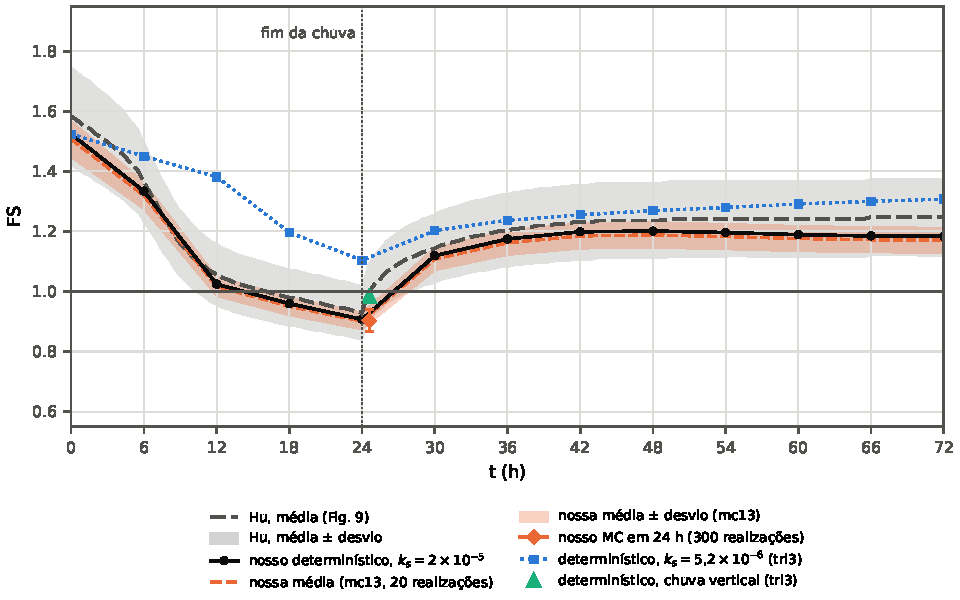
\includegraphics[width=0.9\linewidth]{figs/fig_fig9.pdf}
\caption{FS no tempo a 50~mm/h por 24~h, sobre a Fig.~9 de Hu (média e média $\pm$ desvio das 180 análises do PDEM).
A faixa de Hu é $\approx 2{,}6$ vezes mais larga que a nossa (mc13). O losango em 24~h é a média $\pm$ desvio do MC
direto (300 realizações).}
\label{fig:fig9}
\end{figure}

\begin{figure}[htbp]\centering
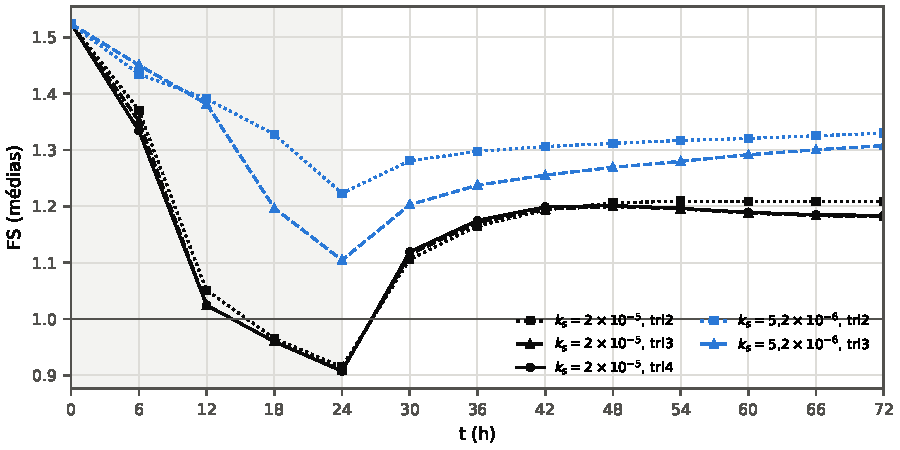
\includegraphics[width=0.75\linewidth]{figs/fig_malha.pdf}
\caption{FS determinístico a 50~mm/h por 24~h nas três malhas do transiente e com os dois $k_s$. A faixa cinza é a
chuva.}
\label{fig:malha}
\end{figure}

\begin{figure}[htbp]\centering
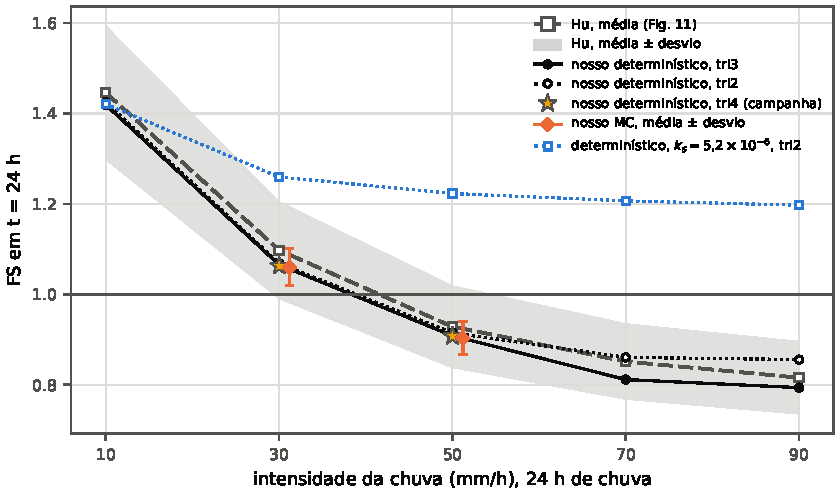
\includegraphics[width=0.72\linewidth]{figs/fig_fig11.pdf}
\caption{FS em 24~h (24~h de chuva) por intensidade, sobre a Fig.~11 de Hu (média e média $\pm$ desvio). As estrelas
são o determinístico da campanha (tri4); os losangos, a média $\pm$ desvio do nosso MC.}
\label{fig:fig11}
\end{figure}

\begin{figure}[htbp]\centering
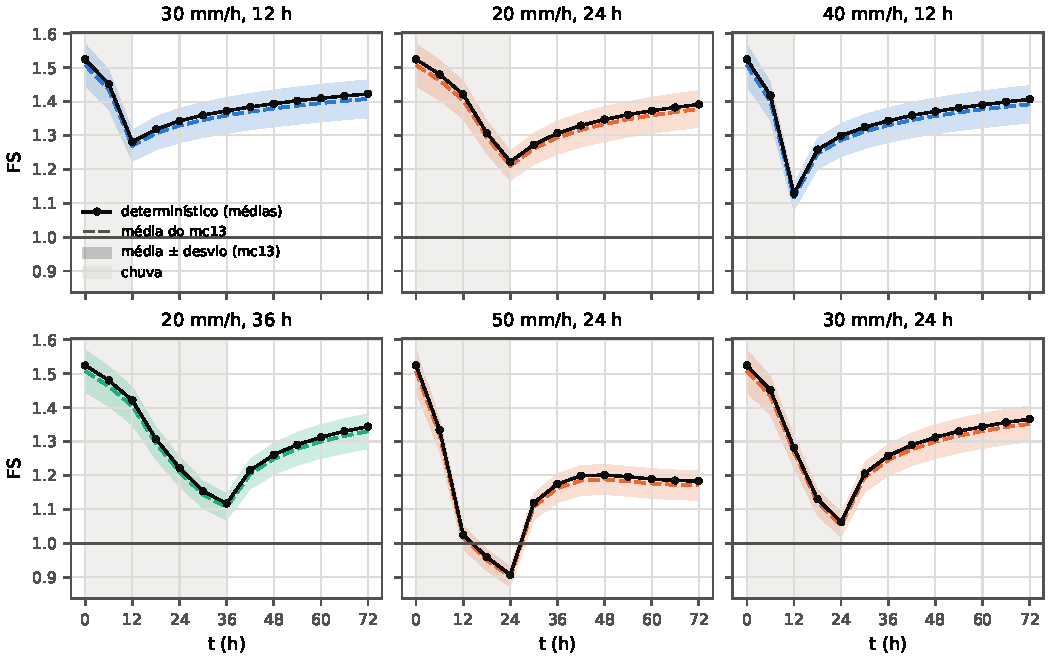
\includegraphics[width=\linewidth]{figs/fig_fs_t.pdf}
\caption{FS no tempo nos \nCasos{} cenários: o determinístico (médias, tri4) e a média $\pm$ desvio das 20 realizações
do mc13. A cor segue a duração da chuva (faixa cinza).}
\label{fig:fs_t}
\end{figure}

\clearpage
\section{Resultados probabilísticos por cenário}\label{sec:prob}
% gerado por gera_dados.py; nao edite
\begin{table}[htbp]\centering\footnotesize\setlength{\tabcolsep}{3pt}
\caption{$P(FS < 1)$ por cenário (primeira passagem até 72~h, em \%; abaixo de $10^{-4}$, em fração). FORM: $\beta$ e $\Phi(-\beta)$ (* = parou nas 10 iterações sem convergir). LS: line sampling na direção do FORM, com o $CoV$ e o IC de 95\,\% normal. MC: Monte Carlo direto, IC de Wilson. $z$: LS contra MC. Hu: Figs.~16 e 19 (0,7781 impresso).}\label{tab:pf}
\begin{tabular}{lrrrrrrrrrr}\toprule
 & \multicolumn{2}{c}{FORM} & \multicolumn{3}{c}{LS} & \multicolumn{3}{c}{MC} & & Hu \\\cmidrule(lr){2-3}\cmidrule(lr){4-6}\cmidrule(lr){7-9}
cenário & $\beta$ & $P_f$ & $P_f$ & $CoV$ & IC 95\,\% & $n_f/N$ & $P_f$ & IC 95\,\% & $z$ & $P_f$ \\\midrule
30 mm/h, 12 h & 10{,}68* & $6{,}2\times 10^{-27}$ & $3{,}0\times 10^{-17}$ & 67{,}3 & -- & 0/500 & 0 & [0; 0{,}762] & -- & 1{,}2 \\
20 mm/h, 24 h & 6{,}46* & $5{,}3\times 10^{-11}$ & $1{,}2\times 10^{-8}$ & 54{,}5 & -- & 0/500 & 0 & [0; 0{,}762] & -- & 3{,}0 \\
40 mm/h, 12 h & 3{,}67* & 0{,}012 & 0{,}072 & 11{,}8 & [0{,}055; 0{,}089] & 5/4000 & 0{,}125 & [0{,}053; 0{,}292] & $-0{,}9$ & 9{,}1 \\
20 mm/h, 36 h & 2{,}84 & 0{,}223 & 0{,}268 & 4{,}9 & [0{,}242; 0{,}293] & 13/4000 & 0{,}325 & [0{,}190; 0{,}555] & $-0{,}6$ & 11{,}70 \\
50 mm/h, 24 h & $-$3{,}09* & 99{,}90 & 99{,}77 & 0{,}04 & [99{,}69; 99{,}85] & 299/300 & 99{,}67 & [98{,}14; 99{,}94] & $+0{,}3$ & 77{,}81 \\
30 mm/h, 24 h & 1{,}50* & 6{,}70 & 7{,}12 & 4{,}7 & [6{,}46; 7{,}78] & 135/2000 & 6{,}75 & [5{,}73; 7{,}93] & $+0{,}6$ & 22{,}10 \\
\bottomrule\end{tabular}\end{table}

\begin{itemize}
  \item \textbf{30~mm/h por 12~h e 20~mm/h por 24~h:} $\beta$ de 10,7 e 6,5. O LS dá $P_f$ de $10^{-17}$ e $10^{-8}$
    (com $CoV$ de 55 a 67\,\% nas 60 linhas do teto), e o MC não tem falha em 500 realizações. Hu dá 1,2 e 3,0\,\%.
    No I30\_D12, uma linha atingiu o teto da raiz ($c = \linhaTeto$), sem efeito na $P_f$.
  \item \textbf{40~mm/h por 12~h:} o LS dá $\pfLSQuarenta\,\%$ ($CoV = \cvLSQuarenta\,\%$ nas 600 linhas do teto). O
    MC dá $\pfMCQuarenta\,\%$ (\nfMCQuarenta{} falhas em 4000), e Hu dá 9,1\,\%. O FORM não convergiu e dá
    $\pfFORMQuarenta\,\%$, seis vezes abaixo do LS. As raízes das linhas variam muito em torno do $\beta$
    (Fig.~\ref{fig:raizes}): o estado limite é curvo nesse cenário.
  \item \textbf{20~mm/h por 36~h:} o único FORM que convergiu ($\beta = 2{,}84$, $P_f = 0{,}223\,\%$). O LS dá
    $\pfLSTrintaSeis\,\%$ e o MC dá $\pfMCTrintaSeis\,\%$. Hu dá 11,7\,\%, 44 vezes mais.
  \item \textbf{50~mm/h por 24~h:} as médias já falham ($\beta < 0$). O LS dá $\pfLSCinquenta\,\%$ e o MC dá
    $\pfMCCinquenta\,\%$, contra 77,81\,\% impressos por Hu: com o nosso desvio, quase toda realização fica abaixo de 1.
  \item \textbf{30~mm/h por 24~h:} o cenário posto na campanha para o MC conferir o LS com $CoV$ de 8\,\%. O LS dá
    $\pfLSTrinta\,\%$ e o MC dá $\pfMCTrinta\,\%$, contra 22,1\,\% de Hu.
  \item \textbf{O FORM:} parou nas 10 iterações em 5 dos 6 cenários. Mesmo assim, o $\beta$ ficou perto do centro das
    raízes do LS (Fig.~\ref{fig:raizes}), e o LS na direção dele é não viesado (Seção~\ref{sec:lsmc}). A importância
    fica quase toda em $\varphi'$ ($\alpha^2_{\varphi} = 0{,}92$ a $0{,}97$).
\end{itemize}

\begin{figure}[htbp]\centering
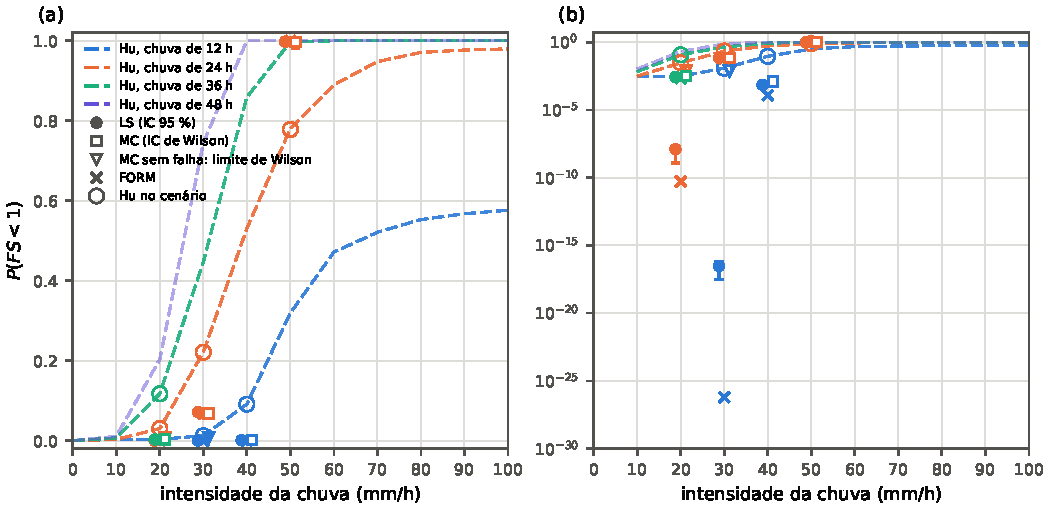
\includegraphics[width=\linewidth]{figs/fig_fragilidade.pdf}
\caption{Fragilidade: as curvas de Hu (Figs.~16 e 19, por duração da chuva) e as nossas $P_f$ nos \nCasos{} cenários,
pelo LS (IC de 95\,\%), pelo MC (IC de Wilson; triângulo: o limite superior quando não há falha) e pelo FORM. O
círculo vazio é a $P_f$ de Hu no cenário. (a) escala linear; (b) escala logarítmica. O FORM de 30~mm/h por 12~h
($6 \times 10^{-27}$) aparece só em (b).}
\label{fig:frag}
\end{figure}

\begin{figure}[htbp]\centering
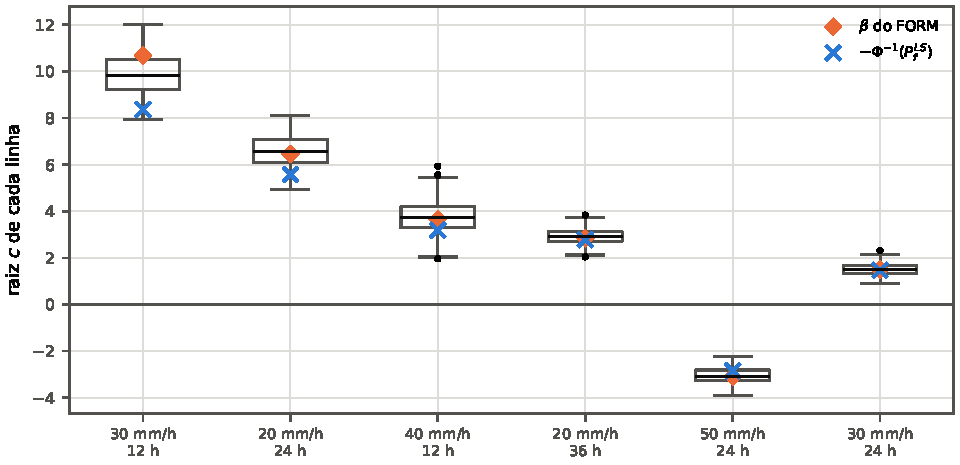
\includegraphics[width=0.85\linewidth]{figs/fig_raizes.pdf}
\caption{As raízes $c$ das linhas do LS por cenário (caixas), o $\beta$ do FORM e o índice equivalente do LS,
$-\Phi^{-1}(P_f^{LS})$.}
\label{fig:raizes}
\end{figure}

\clearpage
\section{O LS contra o MC direto}\label{sec:lsmc}
\begin{itemize}
  \item \textbf{Nos \nZ{} cenários com falhas no MC, o LS fica a menos de um desvio combinado do MC} ($|z| \le
    \zMax$, Tabela~\ref{tab:pf}). Nos outros dois, o MC sem falha só limita a $P_f$ a menos de 0,76\,\%, o que o LS
    confirma com folga.
  \item \textbf{30~mm/h por 24~h (Fig.~\ref{fig:conv}a):} o LS dá $\pfLSTrinta\,\%$ ($CoV = \cvLSTrinta\,\%$) com
    \linhasTrinta{} linhas e \anLSTrinta{} análises. O MC dá $\pfMCTrinta\,\%$ (\nfMCTrinta{} falhas em \nMCTrinta{}),
    e $z = \zTrinta$. Para o mesmo $CoV$ do LS, o MC direto precisaria de $\approx \nMCEquivTrinta$ realizações,
    \razaoTrinta{} vezes o custo do LS.
  \item \textbf{20~mm/h por 36~h (Fig.~\ref{fig:conv}b):} o LS dá $\pfLSTrintaSeis\,\%$ ($CoV =
    \cvLSTrintaSeis\,\%$) com \linhasTrintaSeis{} linhas e \anLSTrintaSeis{} análises. O MC dá
    $\pfMCTrintaSeis\,\%$ (\nfMCTrintaSeis{} falhas em \nMCTrintaSeis{}), e $z = \zTrintaSeis$. Para o mesmo $CoV$, o
    MC direto precisaria de $\approx \nMCEquivTrintaSeis$ realizações, \razaoTrintaSeis{} vezes o custo do LS.
  \item O método, portanto, funciona na chuva como funcionou no Ceron saturado e no Cho seco: a direção do FORM modal,
    mesmo sem convergir, basta para um LS não viesado.
\end{itemize}

\begin{figure}[htbp]\centering
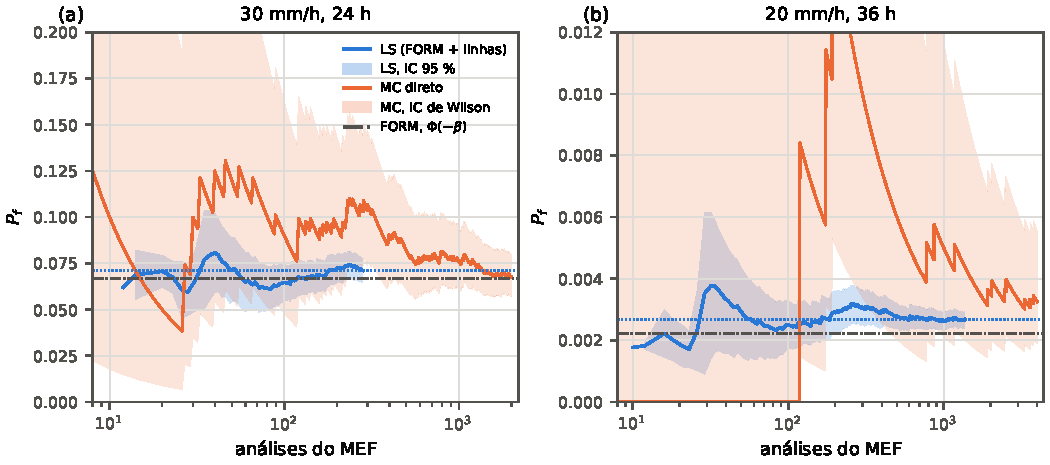
\includegraphics[width=\linewidth]{figs/fig_convergencia.pdf}
\caption{Convergência do LS e do MC direto contra o número de análises do MEF (o LS conta também as do FORM). Faixas:
IC de 95\,\% do LS (normal) e do MC (Wilson). Linhas horizontais: o LS final (pontilhada) e o FORM (traço e ponto).}
\label{fig:conv}
\end{figure}

\section{Por que a nossa $P_f$ difere da de Hu}\label{sec:porque}
\begin{itemize}
  \item \textbf{O desvio do FS (Tabela~\ref{tab:desvio}):} a média do nosso FS fica perto da de Hu, mas o desvio é
    $\approx \razaoSdZero$ do dele: $\sdZero$ contra $\huSdZero$ em 0~h, e $\sdVinteMC$ contra $\huSdVinte$ em 24~h
    (razão $\razaoSdVinte$). Nos nossos \nCasos{} cenários, o $CoV$ do FS no fim da chuva fica entre \cvNossoMin{} e
    \cvNossoMax\,\%. O de Hu fica perto de 10\,\% em todas as intensidades (Tabela~\ref{tab:normal}).
  \item \textbf{O limite homogêneo:} se $c'$ e $\varphi'$ forem variáveis aleatórias (sem campo: o limite de
    correlação infinita, que com essas marginais é, em geral, o de maior desvio), o $CoV$ do FS é de \cvHomZero\,\% em 0~h
    e \cvHomVinte\,\% em 24~h. O de Hu é \cvHuZero{} e \cvHuVinte\,\%, acima desse limite. O cálculo usa o fato de que
    o FS do SRM é homogêneo de grau 1 em $(c', \tan\varphi')$: $FS = \tan\varphi'\, g(c'/\tan\varphi')$. A função $g$
    vem de 11 determinísticos com $\varphi' = 24^\circ$ (\path{~/projects/runs/hu2024/homogeneo}), e a média e o desvio,
    de 400\,000 pares log-normais com $\rho = -0{,}5$. O peso de $c'$ no FS das médias é $w_c = \wcZero$ em 0~h e
    $\wcVinte$ em 24~h. Campos com correlação finita têm, em geral, desvio menor que esse: a média local
    sobre a superfície de ruptura tira variância. Com 150 termos, que cortam 13\,\% da variância, o desvio fica menor
    ainda. A Fig.~\ref{fig:hist}b mostra as três densidades a 50~mm/h por 24~h. Com
    $P_f = \pfHomVinte\,\%$ nesse cenário, nem o limite homogêneo chega aos 77,8\,\% de Hu.
  \item \textbf{O que o desvio de Hu pode ter:} ele não vem dos parâmetros publicados. Pode vir do PDEM: 180 pontos
    escolhidos pelo método da teoria dos números para gerar os 300 coeficientes de KL (150 por campo), cada um
    com a sua probabilidade atribuída, e um desvio ponderado de um jeito que o artigo não descreve. Pode vir também de campos gerados com outra variância (por
    exemplo, $CoV$ aplicado ao campo normal e não ao log-normal) ou de um passo do SLOPE/W que não está descrito. Sem as
    180 histórias de FS, não há como separar essas causas.
  \item \textbf{A aproximação normal (Tabela~\ref{tab:normal}):} $P_f \approx \Phi\bigl((1 - \mu)/\sigma\bigr)$ no fim
    da chuva reproduz a $P_f$ de cada lado com a média e o desvio do próprio lado. Para Hu, dá $\huNormalCinquenta\,\%$
    a 50~mm/h (contra 77,8\,\%) e $\huNormalTrinta\,\%$ a 30~mm/h (contra 22,1\,\%). Para nós, dá
    $\nossoNormalTrinta\,\%$ a 30~mm/h por 24~h, contra $\pfLSTrinta\,\%$ do LS. Com a nossa média e o desvio de Hu, a
    $P_f$ volta à ordem da dele (última coluna). A diferença de $P_f$ é, portanto, quase toda a diferença de desvio:
    nem a média do FS nem o método de confiabilidade explicam.
  \item \textbf{A cauda:} longe da média (30~mm/h por 12~h, 40~mm/h por 12~h e 20~mm/h por 36~h), a aproximação normal
    erra a nossa $P_f$ para cima. A cauda inferior do FS é mais curta que a normal, e o LS mede isso diretamente.
\end{itemize}

% gerado por gera_dados.py; nao edite
\begin{table}[htbp]\centering\footnotesize
\caption{Média, desvio e $CoV$ do FS a 50~mm/h por 24~h, em 0~h e no fim da chuva: os nossos campos (0~h: as 20 realizações do mc13, com o IC de 95\,\% do desvio; 24~h: as 300 do MC), o limite homogêneo ($c'$ e $\varphi'$ como variáveis aleatórias, com os mesmos parâmetros) e Hu (Fig.~9).}\label{tab:desvio}
\begin{tabular}{lrrrrrr}\toprule
 & \multicolumn{3}{c}{0 h} & \multicolumn{3}{c}{24 h} \\\cmidrule(lr){2-4}\cmidrule(lr){5-7}
 & $\mu$ & $\sigma$ & $CoV$ (\%) & $\mu$ & $\sigma$ & $CoV$ (\%) \\\midrule
campos de Nyström ($M = 150$) & 1{,}507 & 0{,}062 [0{,}047; 0{,}091] & 4{,}1 & 0{,}903 & 0{,}036 & 4{,}0 \\
limite homogêneo & 1{,}526 & 0{,}122 & 8{,}0 & 0{,}906 & 0{,}058 & 6{,}5 \\
Hu (Fig.~9) & 1{,}583 & 0{,}165 & 10{,}4 & 0{,}929 & 0{,}091 & 9{,}8 \\
\bottomrule\end{tabular}\end{table}

% gerado por gera_dados.py; nao edite
\begin{table}[htbp]\centering\footnotesize
\caption{A aproximação normal $P_f \approx \Phi\bigl((1 - \mu)/\sigma\bigr)$ com a média e o desvio do FS no fim da chuva. Em cima, Hu: $\mu$ e $\sigma$ da Fig.~11 (24~h de chuva) contra a $P_f$ das Figs.~16 e 19. Embaixo, este trabalho: $\mu$ e $\sigma$ do MC direto contra o LS e o MC. A última coluna põe o desvio de Hu na nossa média.}\label{tab:normal}
\begin{tabular}{lrrrrrr}\toprule
cenário & $\mu$ & $\sigma$ & $CoV$ (\%) & $\Phi\bigl((1 - \mu)/\sigma\bigr)$ & $P_f$ & nossa $\mu$, $\sigma$ de Hu \\\midrule
\multicolumn{7}{l}{\textit{Hu et al.\ (2024), 24~h de chuva}} \\
10 mm/h, 24 h & 1{,}446 & 0{,}148 & 10{,}2 & 0{,}1 & 0{,}3 & -- \\
30 mm/h, 24 h & 1{,}097 & 0{,}107 & 9{,}8 & 18{,}2 & 22{,}1 & -- \\
50 mm/h, 24 h & 0{,}928 & 0{,}091 & 9{,}8 & 78{,}5 & 77{,}8 & -- \\
70 mm/h, 24 h & 0{,}851 & 0{,}084 & 9{,}8 & 96{,}2 & 94{,}8 & -- \\
90 mm/h, 24 h & 0{,}815 & 0{,}081 & 9{,}9 & 98{,}9 & 97{,}7 & -- \\
\midrule\multicolumn{7}{l}{\textit{este trabalho (MC; $P_f$ do LS e, entre parênteses, do MC)}} \\
30 mm/h, 12 h & 1{,}276 & 0{,}052 & 4{,}1 & $6{,}7\times 10^{-8}$ & $3{,}0\times 10^{-17}$ (0) & -- \\
20 mm/h, 24 h & 1{,}217 & 0{,}051 & 4{,}2 & $1{,}0\times 10^{-5}$ & $1{,}2\times 10^{-8}$ (0) & 4{,}5 \\
40 mm/h, 12 h & 1{,}124 & 0{,}042 & 3{,}8 & 0{,}170 & 0{,}072 (0{,}125) & -- \\
20 mm/h, 36 h & 1{,}113 & 0{,}043 & 3{,}9 & 0{,}434 & 0{,}268 (0{,}325) & -- \\
50 mm/h, 24 h & 0{,}903 & 0{,}036 & 4{,}0 & 99{,}62 & 99{,}77 (99{,}67) & 85{,}8 \\
30 mm/h, 24 h & 1{,}060 & 0{,}041 & 3{,}8 & 7{,}06 & 7{,}12 (6{,}75) & 28{,}9 \\
\bottomrule\end{tabular}\end{table}


\begin{figure}[htbp]\centering
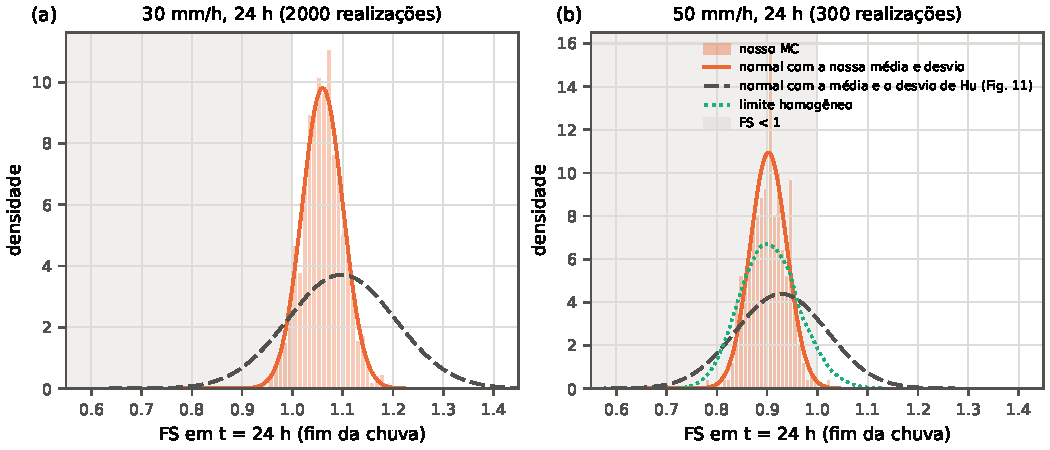
\includegraphics[width=\linewidth]{figs/fig_hist.pdf}
\caption{FS no fim da chuva no MC direto, contra a normal com a nossa média e desvio, a normal com a média e o desvio
de Hu (Fig.~11) e, em (b), a densidade do limite homogêneo. A faixa cinza é a falha.}
\label{fig:hist}
\end{figure}

\clearpage
\section{A primeira passagem}\label{sec:passagem}
\begin{itemize}
  \item A campanha calcula o FS só no fim da chuva $D$ e em $D + 6$~h, porque o determinístico e o piloto de 22/11 dão
    o menor FS em $t = D$, como diz Hu (``the FOS reaches minimum value when the rainfall stop'').
  \item A conferência mc13 mede isso: nas \mcTrezeN{} primeiras realizações de cada cenário, com o FS de 6 em 6~h de 0
    a 72~h, o menor FS da história cai em $t = D$ em \mcTrezeN{} de \mcTrezeN{}, nos \mcTrezeOk{} cenários. A maior
    diferença entre o FS em $D$ e o menor da história é $\mcTrezeDif$ (Fig.~\ref{fig:fs_t}).
  \item A falha de primeira passagem até 72~h é, então, a falha no fim da chuva, e a $P_f$ da campanha é a mesma
    grandeza das Figs.~16 e 19 de Hu.
\end{itemize}

\section{Conclusões e próximos passos}\label{sec:conclusoes}
\begin{itemize}
  \item \textbf{Determinístico:} o modelo reproduz a média do FS de Hu no tempo e por intensidade, de 2 a 5\,\% abaixo
    (SRM contra equilíbrio limite), com o $k_s$ do texto ($2 \times 10^{-5}$~m/s). O $k_s$ da Fig.~4b não reproduz. A
    malha tri4 é a necessária.
  \item \textbf{Método:} o LS na direção do FORM modal concorda com o MC direto em todos os cenários em que o MC
    mede ($|z| \le \zMax$). Para o mesmo $CoV$, ele custa de \razaoTrinta{} a \razaoTrintaSeis{} vezes menos que o MC, mesmo com o FORM sem
    convergir.
  \item \textbf{$P_f$:} as de Hu não se reproduzem a partir dos dados publicados. O desvio do FS dele passa do limite
    homogêneo, e a média e o desvio dele, na aproximação normal, já dão a $P_f$ dele. Hu fica como verificação
    determinística e como problema de teste do LS contra o nosso MC. As referências de $P_f$ da literatura passam a ser
    os casos B (Liu et al.~2024) e C (Liu e Wang 2023).
  \item \textbf{Próximos passos:}
    \begin{itemize}
      \item o caso B (Liu et al.\ 2024) já está no fermi (campanha \texttt{liu2024}: FORM modal, LS e MC direto nos
        cenários 2 e 3); o C espera a decisão sobre a campanha (\texttt{FORCAR=1});
      \item o ar ativo nos mesmos campos: rodar o caso A com o modelo acoplado água--ar, pareado com este (ar
        passivo), para medir o efeito do ar na $P_f$ com os mesmos números aleatórios;
      \item perguntar a Hu e Bao o $k_s$ que rodou, como os 180 pontos do PDEM geram os 300 coeficientes e as 180
        histórias de FS;
      \item opcional: um MC com $M = 200$ ou com o campo inteiro, para medir quanto os 13\,\% de variância cortados
        pesam (pouco: mesmo o limite homogêneo fica longe de Hu).
    \end{itemize}
\end{itemize}

\begin{thebibliography}{9}
\bibitem{hu2024} H.~Hu, Y.~Bao, X.~Han, W.~Wang. Non-parametric fragility curves for probabilistic risk assessment
  of rainfall-triggered landslides. \emph{Computers and Geotechnics}, 173:106546, 2024.
  doi:10.1016/j.compgeo.2024.106546.
\bibitem{cho2010} S.~E.~Cho. Probabilistic assessment of slope stability that considers the spatial variability of
  soil properties. \emph{Journal of Geotechnical and Geoenvironmental Engineering}, 136(7):975--984, 2010.
\bibitem{hasofer1974} A.~M.~Hasofer, N.~C.~Lind. Exact and invariant second-moment code format. \emph{Journal of the
  Engineering Mechanics Division (ASCE)}, 100(1):111--121, 1974.
\bibitem{rackwitz1978} R.~Rackwitz, B.~Fiessler. Structural reliability under combined random load sequences.
  \emph{Computers \& Structures}, 9(5):489--494, 1978.
\bibitem{koutsourelakis2004} P.~S.~Koutsourelakis, H.~J.~Pradlwarter, G.~I.~Schuëller. Reliability of structures in
  high dimensions, part~I: algorithms and applications. \emph{Probabilistic Engineering Mechanics}, 19(4):409--417,
  2004. doi:10.1016/j.probengmech.2004.05.001.
\bibitem{wilson1927} E.~B.~Wilson. Probable inference, the law of succession, and statistical inference.
  \emph{Journal of the American Statistical Association}, 22(158):209--212, 1927.
\bibitem{formulacao} Campos aleatórios e confiabilidade de taludes: as bases de Karhunen--Loève (analítica e Nyström),
  o FORM com gradiente modal (SRM e GIM) e o line sampling. Documento interno,
  \path{docs/confiabilidade_campos/formulacao/formulacao.pdf}, 2026.
\bibitem{exemplos} Exemplos probabilísticos de chuva não saturada (a especificação dos casos A, B e C). Relatório
  interno, \path{~/Dropbox/UnsaturatedSoil/referencias/referencias_selecionadas_claude/reports/}, 2026.
\end{thebibliography}

\appendix
\section{Arquivos e como refazer}
\begin{itemize}
  \item \textbf{A especificação} do caso A é a seção ``A)'' do relatório dos exemplos~\cite{exemplos}; as curvas de
    Hu lidas dos vetores do PDF estão em \path{reports/figs/dados} (\texttt{hu\_fig9\_media\_dp.csv},
    \texttt{hu\_fig11\_fs24.csv}, \texttt{hu\_fragilidade.csv}).
  \item \textbf{A campanha:} \path{Projects/SlopeRandomFieldRefinement/cluster/hu2024_casos.sbatch}, com os cenários
    em \path{casos_hu2024.txt}; saída no fermi em \path{$DATA/hu2024_ks2e-5}, baixada em
    \path{~/projects/runs/fermi_hu2024_ks2e-5}.
  \item \textbf{As conferências no PC:} \path{~/projects/runs/hu2024} (\path{det/}: os dois $k_s$, as malhas, a chuva
    vertical e o FS em 24~h por intensidade; \path{piloto/}; \path{nystrom/}; \path{gradiente/}; \path{form/};
    \path{homogeneo/roda.sh}: o limite homogêneo).
  \item \textbf{Este relatório:} \texttt{gera.sh} refaz o resumo (\texttt{resumo\_hu2024.py}) sobre a campanha baixada,
    roda o \texttt{gera\_dados.py} (tabelas em \path{tab/}, números em \path{numeros.tex}, figuras em \path{figs/}) e
    o \LaTeX.
\end{itemize}
\end{document}
